% !TeX spellcheck = fr-moderne
\section{Introduction de l'industrie de la télécommunication}
\subsection{L'evolution des normes de téléphonie mobile}
Depuis 1984, il y a déjà plusieurs standards ont été utilisé par les opérateur dans le monde entier. Voici un tableau de différentes standards mobile en Europe et ses paramétrés \ref{tbl:GMIE}. 
\begin{table}[H]
\begin{tabular}{|p{2cm}|p{2cm}|p{2cm}|p{4cm}|}
	\hline
	Génération&Acronyme&Description&Débit\\
	\hline
	1G		&Radiocom 2000	&Échanges de type voix uniquement&analogique\\
	\hline
	\hline
	2G		&GSM			&Échanges de type voix uniquement	&9,05 kbps\\
	\hline
	2,5G	&GPRS			&Échange de données sauf voix		&171,2 kbps / 50 kbps / 17,9 kbps\\
	\hline
	\hline
	3G		&UMTS			&Voix + données						&144 kbps rurale, 384 kbps urbaine, 1,9 Mbps point fixe / -\\
	\hline
	3.5G ou 3G+ ou H&HSPA	&Évolution de l'UMTS				&14,4 Mbps / 3,6 Mbps / -\\
	\hline
	\hline
	4G		&LTE			&Long Term Evolution (Données)				&150 Mbps / 40 Mbps / -\\
	\hline
	4G		&LTE-Advanced	&Long Term Evolution Advanced (Données+voix)		&1 Gbps à l'arrêt, 100 Mbps en mouvement / - / -\\
	\hline
\end{tabular}
\caption{Les différentes générations de téléphonie mobile en Europe}
 \label{tbl:GMIE}
\end{table}

\subsubsection{La premier génération}
En télécommunication, \textsf{1G} est la premier génération des standards pour la téléphonie mobile, il s'agit de la première apparition du réseaux de téléphonie mobile, 1G sont des réseaux analogiques, peut échanges de type voix uniquement.
\subsubsection{La deuxième génération}
\textsf{2G}, la technologie de téléphonie sans fil de deuxième génération, la différence entre le réseaux 1G et 2G est: le signaux radio sur les réseaux 1G sont analogiques, et celle de 2G sont numériques.

Systèmes 2G ont été significativement plus efficaces du spectre permettant de bien plus grand taux de pénétration du téléphone mobile, en plus les données vocales numériques peuvent être compressées et multiplexées beaucoup plus efficacement que les codages de la voix analogique grâce à l'utilisation de codecs différents, ce qui permet plus d'appels à transmettre dans la même quantité de bande passante radio. Et 2G présenté premier foi les services de données pour mobile. Les Technologie 2G permettent les divers réseaux de téléphonie mobile de utiliser des services tels que le SMS et MMS. Tous les message de texte envoyés au delà de 2G sont chiffrés numériquement, ce qui permet le transfert de données de telle sorte que seul le destinataire peut recevoir et lire.   

Réseaux 2G ont été construits principalement pour les services téléphoniques et de transmission de données lent (défini dans les documents de spécifications IMT-2000).

Réseaux \textsf{2,5G}, on le qualifie souvent de le General packet Radio Service ou GPRS, est une norme pour la téléphonie mobile dérivée du GSM et complémentaire de celui-ci, permettant un débit de données plus élevé. Le 2,5 indique que c'est une technologie à mi-chemin entre le GSM (deuxième génération) et l'UMTS (troisième génération). Le GPRS est une extension du protocole GSM : il ajoute par rapport à ce dernier la transmission par paquets. Cette méthode est plus adaptée à la transmission des données. En effet, les ressources ne sont allouées que lorsque des données sont échangées, contrairement au mode « circuit » en GSM où un circuit est établi – et les ressources associées – pour toute la durée de la communication. Le GPRS a ensuite évolué au début des années 2000 vers la norme \textsc{edge} également optimisée pour transférer des données et qui utilise les mêmes antennes et les mêmes fréquences radio.
\subsubsection{La troisième génération}
La troisième génération (3G) des normes de téléphonie mobile. Elle est représentée principalement par W-CDMAmm, CDMA2000, TD-SCDMA et WiMAX. Elle permettant des débits de 2 à 42 Mb/s qui sont bien plus rapides qu'avec la génération précédente. Grâce à l'utilisation des règles de classement utilisateur, et les  bandes de fréquences supérieures rendant la capacité du réseau augmenter.

Dans les différentes standard  3G et ses prédécesseur, ils utilisent le domaine CS (Circuit Switch)  pour les services vocaux, et le domaine PS (Packet Switch) s'occupe des services de données \ref{Fig.3G.1}.
\subsubsection{La quatrième génération}
La quatrième génération des standards pour la téléphonie mobile, succédant à la 2G et la 3G, en théorie, elle permet de transmette de données à des débits supérieur à 100 Mb/s. 

Une des particularité de la 4G est sa EPC (Evolved Packet Core) est basé sur IP, et il n'y a plus de mode commuté (le 'Circuit Switched Domain' qui s'occupe le service vocaux dans les standard précédant), ce qui signifie que les services vocaux transmis sur l'internet \ref{Fig.3G.2}. 


\begin{figure}[H]
	\centering
	\subfigure[Réseau 3G et ses prédécesseur]{
		\label{Fig.3G.1}
		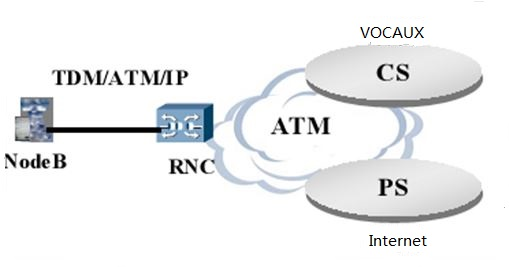
\includegraphics[width=3in]{images/3G2.JPG}}\hfill		
	\hspace{1in}
%\flushright
	\subfigure[Réseau 4G]{
		\label{Fig.3G.2}
		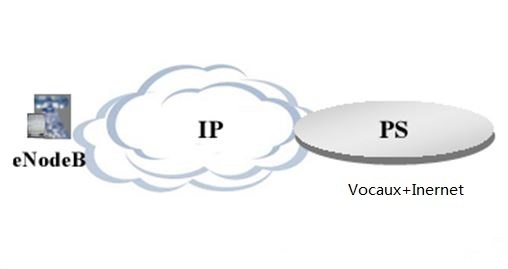
\includegraphics[width=3in]{images/4g.JPG}}
	\caption{Structure des réseaux} 
		\label{Fig.3G}
\end{figure}

\subsection{Le réseau LTE}
Le LTE (Long Term Evolution) est l'evolution la plus récent des normes de CDMA 2000, TD-SCDMA, GSM. La norme LTE. La technologie LTE été considérée comme une norme de troisième génération '3.9G', et la 'vraie 4G', appelée LTE-Advanced été reconnu par l'UIT comme une technologie 4G en 2010. LTE a deux branche: LTE-FDD (Frequency-Division Duplex  Long Term Evolution)et LTE-TDD, (Time Division Duplex Long Term Evolution)les deux standards sont similaire \ref{evolution}. En 2011-2012, les réseaux LTE-TDD sont commercialisés sous l'appellation 4G par CMCC un Chine.
      \begin{figure}[H]
          \centering
          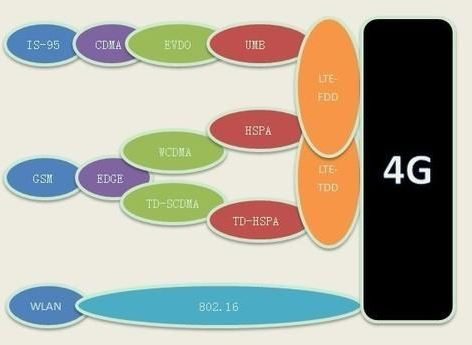
\includegraphics[width=4in]{images/evolution.JPG}
          \caption{l'evolution des standard}
          \label{evolution}
      \end{figure}
      
\subsubsection{La structure du réseau LTE}
Le réseau 4G contient 2 partie: eNodeB (le station), EPC (Evolved Packet Core) qui contient MME, S-GW, P-GW et HSS \ref{structure4G}  \ref{founction du chaque partie}. 
    
      \begin{figure}[H]
          \centering
          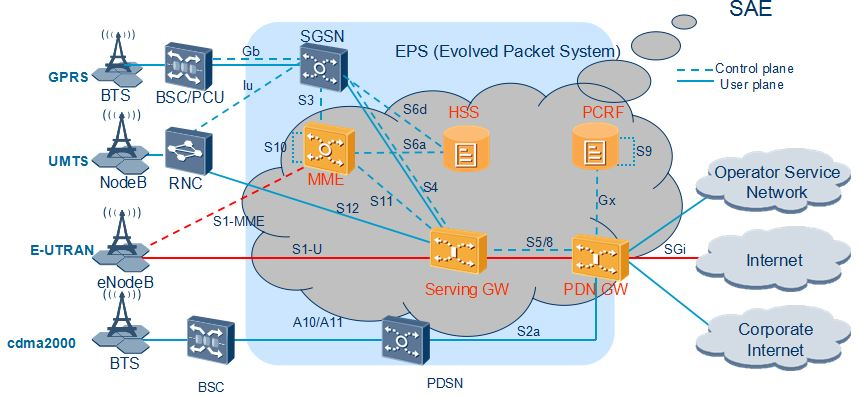
\includegraphics[width=5in]{images/enb2.jpg}
          \caption{la structure du réseau}
          \label{structure4G}
      \end{figure}
      
\begin{table}[H]
	\begin{tabular}{|p{2cm}|p{11 cm}|}
		\hline Part &                     Fonction\\
		\hline MME & 
			L'authentification des utilisateurs et la gestion des clés,  Cryptage de la couche NAS,  Gestion de la liste TA, Sélection P-GW ou S-GW \\ 
		\hline Service Gateway & Compression d'en-tête IP, Routage de paquets et la transmission, La commutation entre eNB, Facturation des utilisateurs porteur \\ 
		\hline PDN Gateway & L'allocation des adresses IP de UE, l'accès aux fonction de gestion de réseau externes, Facturation en service \\ 
		\hline HSS(Home Subscriber Service) & Stockée données de utilisateur associées au service \\ 
		\hline PCRF & Roaming \\ 
		\hline 
	\end{tabular} 
	\caption{la fonction du chaque partie}
	\label{founction du chaque partie}
\end{table}    

Entre deux \textsc{e-utran}, il y a l'interface X2, l'interface S-11 se trouve entre S-GW et MME, \textsc{e-utran} et S-GW échange les données par l'interface S1-U \ref{Fig.S1}et il échange les donnée par l'interface S1-AP avec MME \ref{Fig.S1}, MME et HSS utilise l'interface S6A, et l'interface S5/8 entre S-GW et P-GW, Gx entre PCRF et P-GW. En mettant des capteur en les interfaces, les opérateurs et les fournisseurs d'équipement peuvent collecter les données de signalisation, et utilisent ces données pour trouver les défauts du système. 
      \begin{figure}[H]
          \centering
          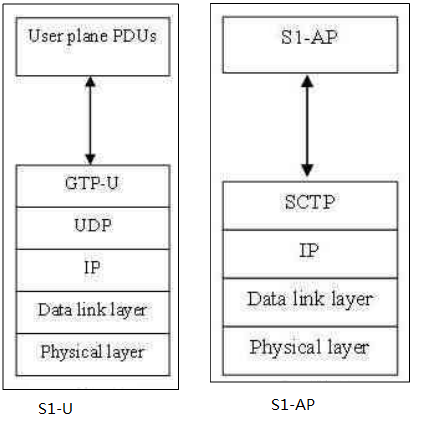
\includegraphics[width=2in]{images/S1-U.png}
          \caption{Interface S1}
          \label{Fig.S1}
      \end{figure}

\section{Introduction des données}

Après quelque semaines de négociation avec les employés de différents départements de la CMCC, ils nous ont fourni deux versions de données, et ses spécifications du format. Nous avons trouvé que CMCC n'a pas de accès direct aux données, et la spécification fourni par  CMCC n'est pas correct, et il y a des erreur dans les données fourni par les fournisseur d'équipement.

Ils nous ont envoyé 11 dossiers, chaque dossier correspond à un service. les services sont 'rtsp', 'dns','mail', 'ftp', 'http-wap', 'mms', 'p2p', 'realtimecom', 'VoIP' et les données de signalisation entre \textsc{e-utran} et MME 'S1AP-NAS'\ref{dossier}. 
      \begin{figure}[H]
          \centering
          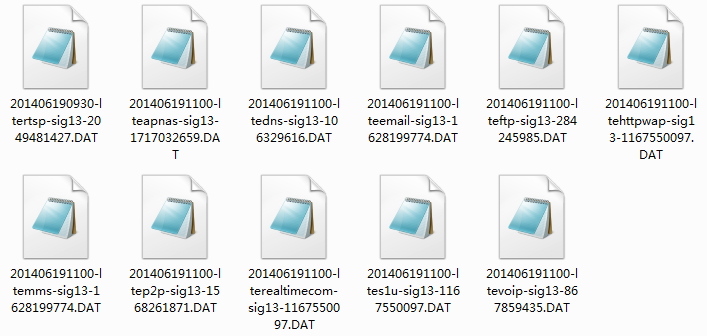
\includegraphics[width=5in]{images/data.png}
          \caption{les dossiers de données}
          \label{dossier}
      \end{figure}
Et nous avons trouvé que pour les services comme 'VoIP' et 'RTSP', ils sont très peu de données \ref{table.nombre}. Donc nous avons décidé de utiliser le donnée du service 'HTTP'.

\begin{table}[H]
\centering
	\begin{tabular}{|>{\centering\arraybackslash}p{4 cm}|>{\centering\arraybackslash}p{4 cm}|}
	\hline \textsf{L'interface }& \textsf{Nombre de ligne} \\ 
	\hline S1-AP & 240 \\ 
	\hline RTSP & 35 \\ 
	\hline DNS  & 272562 \\ 
	\hline Maill & 44 \\ 
	\hline FTP & 71 \\ 
	\hline HTTP-WAP & 50854 \\ 
	\hline MMS & 193 \\ 
	\hline P2P & 515 \\ 
	\hline Realtimecom & 2082 \\ 
	\hline S1U & 89759 \\ 
	\hline VoIP & 28 \\ 
	\hline 
	\end{tabular} 
	\caption{les dossiers de données}
	          \label{table.nombre}
\end{table}


\subsection{Prétraitement de données}
Dans le dossier de HTTP, il y a 50854 lignes, chaque ligne a 76 attributs \ref{Fig.HTTP}, les données sont collectent dans 20 minutes.
      \begin{figure}[H]
          \centering
          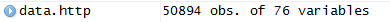
\includegraphics[width=5in]{images/http.png}
          \caption{les données du service HTTP}
          \label{Fig.HTTP}
      \end{figure}

En analysant des données, nous avons trouvé des erreur, et le fournisseur nous a confirmé que ces sont les défaut de leur système 4G. Par exemple, ils sont chiffré les données en utilisant le codage BCD, et Un \ref{fig:errorData}

Deux \ref{fig:défaut}
      \begin{figure}[H]
\centering
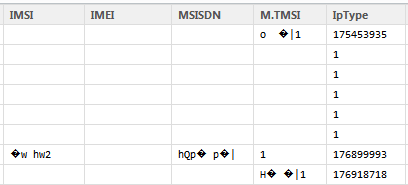
\includegraphics[width=0.7\linewidth]{images/errorData}
\caption{erreur du codage BCD}
\label{fig:errorData}
\end{figure}

      \begin{figure}[H]
\centering
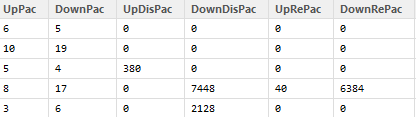
\includegraphics[width=0.7\linewidth]{images/11}
\caption{Défaut de la système}
\label{fig:défaut}
\end{figure}

      